\documentclass[10pt,oneside,openany]{memoir}
%%%%%%%%%%%%%%%%%%%%%%%%%%%%%%%%%%%%%%%%%%%%%%%%%%%%%%%%%%%%%%%%%%%%%%%%%%%%%%%%%%%%%
% Font options
%%%%%%%%%%%%%%%%%%%%%%%%%%%%%%%%%%%%%%%%%%%%%%%%%%%%%%%%%%%%%%%%%%%%%%%%%%%%%%%%%%%%%

\iffalse
%font style 1
\usepackage[p,osf]{scholax}
\usepackage{amsmath,amsthm,amssymb}
\usepackage[scaled=1.075,ncf,vvarbb]{newtxmath}
\fi

%font style2
\usepackage[T1]{fontenc}
\usepackage{amsmath}
\usepackage[fixamsmath]{mathtools}  % Extension to amsmath
\usepackage{amsthm}
\usepackage{amssymb}
\renewcommand*{\mathbf}[1]{\mathbb{#1}}
\renewcommand{\qedsymbol}{$\blacksquare$}

%font style 3
%\usepackage{newpxtext}
%\usepackage{eulerpx}
%\usepackage{mathrsfs}
%\usepackage{eucal}

\usepackage[uprightgreeks,light]{kpfonts}
\usepackage{datetime}
%%%%%%%%%%%%%%%%%%%%%%%%%%%%%%%%%%%%%%%%%%%%%%%%%%%%%%%%%%%%%%%%%%%%%%%%%%%%%%%%%%%%%
% Page layout and headers
%%%%%%%%%%%%%%%%%%%%%%%%%%%%%%%%%%%%%%%%%%%%%%%%%%%%%%%%%%%%%%%%%%%%%%%%%%%%%%%%%%%%%


\usepackage[margin=1in]{geometry}
\usepackage{graphicx} % needed for \scalebox
\usepackage{fancyhdr}
\usepackage{datetime}

\pagestyle{fancy}
\fancyhf{}
\cfoot{\scriptsize\thepage}
\fancyhead[R]{\scalebox{0.8}{\nouppercase{\rightmark}}}
\fancyhead[L]{\scalebox{0.8}{\nouppercase{\leftmark}}}

\fancypagestyle{plain}{%
    \fancyhf{}
    \cfoot{\scriptsize\thepage}
    \fancyhead[R]{\scalebox{0.8}{\phantom{a}}}
    \fancyhead[L]{\scalebox{0.8}{Applied Analysis}}
}

\renewcommand{\headrulewidth}{0pt}
\renewcommand{\footrulewidth}{0pt}

%%%%%%%%%%%%%%%%%%%%%%%%%%%%%%%%%%%%%%%%%%%%%%%%%%%%%%%%%%%%%%%%%%%%%%%%%%%%%%%%%%%%%
% Theorem environments
%%%%%%%%%%%%%%%%%%%%%%%%%%%%%%%%%%%%%%%%%%%%%%%%%%%%%%%%%%%%%%%%%%%%%%%%%%%%%%%%%%%%%

\usepackage{keytheorems}

\newkeytheoremstyle{def}{
    inherit-style=definition,
    spaceabove=1.5em,
    spacebelow=1.5em,
    postheadspace=0.5em,
}

\newkeytheoremstyle{thm}{
    spaceabove=1.5em,
    spacebelow=1.5em,
    postheadspace=0.5em,
}

\newkeytheorem{theorem}[
    name = Theorem,
    style=thm,
    numberwithin = section,
]

\newkeytheorem{theorem*}[
    name=Theorem,
    style=thm,
    numbered=false
]

\newkeytheorem{proposition}[
    name = Proposition,
    style=thm,
    numberwithin = section,
    sibling=theorem
]

\newkeytheorem{lemma}[
    name = Lemma,
    style=thm,
    numberwithin = section,
    sibling=theorem
]

\newkeytheorem{corollary}[
    name = Corollary,
    style=thm,
    numberwithin = section,
    sibling=theorem
]

\newkeytheorem{definition}[
    name = Definition,
    style=def,
    numberwithin = section,
    style = definition
]

\newkeytheorem{example}[
    name = Example,
    style=def,
    numberwithin = section,
    style = definition
]

\newkeytheorem{remark}[
    name=Remark,
    style=remark,
    numbered=false
]

\newkeytheorem{question}[
    name=Question,
    style=remark,
    numbered=false
]

\newkeytheorem{exercise}[
    name = Exercise,
    style=thm
]
\newkeytheorem{problem}[
    name = Problem,
    style=thm
]

\newkeytheorem{axiom}[name = Axiom]

%%%%%%%%%%%%%%%%%%%%%%%%%%%%%%%%%%%%%%%%%%%%%%%%%%%%%%%%%%%%%%%%%%%%%%%%%%%%%%%%%%%%%
% Section and chapter formatting
%%%%%%%%%%%%%%%%%%%%%%%%%%%%%%%%%%%%%%%%%%%%%%%%%%%%%%%%%%%%%%%%%%%%%%%%%%%%%%%%%%%%%

\usepackage{enumitem}
\usepackage[explicit]{titlesec}

\titleformat{\chapter}[display]
    {\bfseries\LARGE\raggedright}
    {Chapter {\thechapter}}
    {.1ex minus .1ex}
    {\Large #1}

\titlespacing{\chapter}
    {3pc}{*3}{40pt}[3pc]

\titleformat{\section}[block]
    {\normalfont\bfseries\large}
    {}{0pt}
    {\fbox{\strut \S\ \thesection.\ #1}}

\titlespacing{\section}
    {0pt}{3ex plus .1ex minus .2ex}{3ex plus .1ex minus .2ex}

\setlength{\fboxsep}{4pt}    % padding inside the box
\setlength{\fboxrule}{0.6pt} % border thickness

\titleformat{name=\section,numberless}[block]
    {\normalfont\bfseries\large\raggedright}
    {}{0pt}
    {\fbox{\strut #1}}

%%%%%%%%%%%%%%%%%%%%%%%%%%%%%%%%%%%%%%%%%%%%%%%%%%%%%%%%%%%%%%%%%%%%%%%%%%%%%%%%%%%%%
% Graphics, symbols, and miscellaneous packages
%%%%%%%%%%%%%%%%%%%%%%%%%%%%%%%%%%%%%%%%%%%%%%%%%%%%%%%%%%%%%%%%%%%%%%%%%%%%%%%%%%%%%

\usepackage{tikz}
\usepackage{tikz-cd}
\usepackage{float}
\usepackage{wasysym}
\usepackage{hyperref}
\usepackage{ulem}
\usepackage{pgfplots}
\usetikzlibrary{patterns}
\usetikzlibrary{positioning,arrows.meta}
\usetikzlibrary{decorations.pathreplacing}
\usetikzlibrary{patterns}
\usepgfplotslibrary{fillbetween}
\pgfplotsset{compat=1.18}
\usepackage{etoolbox}
\usepackage{bm}

%%%%%%%%%%%%%%%%%%%%%%%%%%%%%%%%%%%%%%%%%%%%%%%%%%%%%%%%%%%%%%%%%%%%%%%%%%%%%%%%%%%%%
% Final Formatting/Extra commands
%%%%%%%%%%%%%%%%%%%%%%%%%%%%%%%%%%%%%%%%%%%%%%%%%%%%%%%%%%%%%%%%%%%%%%%%%%%%%%%%%%%%%

\newcommand{\homeworktitle}[3]{%
    \begin{center}
        {\large #1 \\[0.1in] #2}\\[.175in]
        {Name:} {\underline{#3\hspace*{2in}}}\\[0.15in]
    \end{center}
    \vspace{4pt}
}
\newdateformat{specialdate}{\THEYEAR\ \monthname\ \THEDAY}

%%%%%%%%%%%%%%%%%%%%%%%%%%%%%%%%%%%%%%%%%%%%%%%%%%%%%%%%%%%%%
%%%%%%%%%%%%%%%%%%%%%%%%%%%%%%%%%%%%%%%%%%%%%%%%%%%%%%%%%%%%%

% ============================================================
% makros.tex — reorganized, full restored version
% ============================================================

% ============================================================
% Sha / Cyrillic support notes
% ============================================================

%to make the correct symbol for Sha
%\newcommand\cyr{%
%\renewcommand\rmdefault{wncyr}%
%\renewcommand\sfdefault{wncyss}%
%\renewcommand\encodingdefault{OT2}%
%\normalfont \selectfont} \DeclareTextFontCommand{\textcyr}{\cyr}

% ============================================================
% Math operators
% ============================================================

\DeclareMathOperator{\ab}{ab}
\DeclareMathOperator{\ad}{ad}
\DeclareMathOperator{\adj}{adj}
\DeclareMathOperator{\alg}{alg}
\DeclareMathOperator{\Alt}{Alt}
\DeclareMathOperator{\Ann}{Ann}
\DeclareMathOperator{\arith}{arith}
\DeclareMathOperator{\Aut}{Aut}
\DeclareMathOperator{\Be}{B}
\DeclareMathOperator{\Bd}{Bd}
\DeclareMathOperator{\card}{card}
\DeclareMathOperator{\Char}{char}
\DeclareMathOperator{\csp}{csp}
\DeclareMathOperator{\codim}{codim}
\DeclareMathOperator{\coker}{coker}
\DeclareMathOperator{\coh}{H}
\DeclareMathOperator{\compl}{compl}
\DeclareMathOperator{\conj}{conj}
\DeclareMathOperator{\cont}{cont}
\DeclareMathOperator{\Cov}{Cov}
\DeclareMathOperator{\crys}{crys}
\DeclareMathOperator{\Crys}{Crys}
\DeclareMathOperator{\cusp}{cusp}
\DeclareMathOperator{\diag}{diag}
\DeclareMathOperator{\diam}{diam}
\DeclareMathOperator{\Dom}{Dom}
\DeclareMathOperator{\disc}{disc}
\DeclareMathOperator{\dist}{dist}
\DeclareMathOperator{\Div}{div}
\DeclareMathOperator{\dR}{dR}
\DeclareMathOperator{\Eis}{Eis}
\DeclareMathOperator{\End}{End}
\DeclareMathOperator{\ev}{ev}
\DeclareMathOperator{\eval}{eval}
\DeclareMathOperator{\Eq}{Eq}
\DeclareMathOperator{\Ext}{Ext}
\DeclareMathOperator{\Fil}{Fil}
\DeclareMathOperator{\Fitt}{Fitt}
\DeclareMathOperator{\Frob}{Frob}
\DeclareMathOperator{\G}{G}
\DeclareMathOperator{\Gal}{Gal}
\DeclareMathOperator{\GL}{GL}
\DeclareMathOperator{\Gr}{Gr}
\DeclareMathOperator{\Graph}{Graph}
\DeclareMathOperator{\GSp}{GSp}
\DeclareMathOperator{\GUn}{GU}
\DeclareMathOperator{\Hom}{Hom}
\DeclareMathOperator{\id}{id}
\DeclareMathOperator{\Id}{Id}
\DeclareMathOperator{\Ik}{Ik}
\DeclareMathOperator{\IM}{Im}
\DeclareMathOperator{\Image}{im}
\DeclareMathOperator{\Ind}{Ind}
\DeclareMathOperator{\Inf}{inf}
\DeclareMathOperator{\ins}{ins}
\DeclareMathOperator{\inv}{inv}
\DeclareMathOperator{\Isom}{Isom}
\DeclareMathOperator{\J}{J}
\DeclareMathOperator{\Jac}{Jac}
\DeclareMathOperator{\lcm}{lcm}
\DeclareMathOperator{\length}{length}
\DeclareMathOperator*{\limit}{limit}
\DeclareMathOperator{\Log}{Log}
\DeclareMathOperator{\M}{M}
\DeclareMathOperator{\Mat}{Mat}
\DeclareMathOperator{\N}{N}
\DeclareMathOperator{\Nm}{Nm}
\DeclareMathOperator{\NIk}{N-Ik}
\DeclareMathOperator{\NSK}{N-SK}
\DeclareMathOperator{\new}{new}
\DeclareMathOperator{\obj}{obj}
\DeclareMathOperator{\old}{old}
\DeclareMathOperator{\ord}{ord}
\DeclareMathOperator{\Or}{O}
\DeclareMathOperator{\op}{op}
\DeclareMathOperator{\out}{out}
\DeclareMathOperator{\PGL}{PGL}
\DeclareMathOperator{\PGSp}{PGSp}
\DeclareMathOperator{\rank}{rank}
\DeclareMathOperator{\Ran}{Ran}
\DeclareMathOperator{\rel}{Rel}
\DeclareMathOperator{\Real}{Re}
\DeclareMathOperator{\RES}{res}
\DeclareMathOperator{\Res}{Res}
%\DeclareMathOperator{\Sha}{\textcyr{Sh}}
\DeclareMathOperator{\Sel}{Sel}
\DeclareMathOperator{\semi}{ss}
\DeclareMathOperator{\sgn}{sign}
\DeclareMathOperator{\SK}{SK}
\DeclareMathOperator{\SL}{SL}
\DeclareMathOperator{\SO}{SO}
\DeclareMathOperator{\Sp}{Sp}
\DeclareMathOperator{\Span}{span}
\DeclareMathOperator{\Spec}{Spec}
\DeclareMathOperator{\spin}{spin}
\DeclareMathOperator{\st}{st}
\DeclareMathOperator{\St}{St}
\DeclareMathOperator{\SUn}{SU}
\DeclareMathOperator{\supp}{supp}
\DeclareMathOperator{\Sup}{sup}
\DeclareMathOperator{\Sym}{Sym}
\DeclareMathOperator{\Tam}{Tam}
\DeclareMathOperator{\tors}{tors}
\DeclareMathOperator{\tr}{tr}
\DeclareMathOperator{\Tr}{Tr}
\DeclareMathOperator{\un}{un}
\DeclareMathOperator{\Un}{U}
\DeclareMathOperator{\val}{val}
\DeclareMathOperator{\vol}{vol}

% ============================================================
% General aliases and short macros
% ============================================================

\newcommand{\absgal}{\G_{\bbQ}}
\newcommand{\Loc}{L_{\operatorname{loc}}}
\renewcommand{\k}{\kappa}
\newcommand{\Ff}{F_{f}}
%\newcommand{\ts}{\,^{t}\!}
\newcommand{\lat}{\mathscr{L}}
\newcommand{\ov}[1]{\overline{#1}}
\newcommand{\up}{\upsilon}
\newcommand{\e}{\epsilon}
\newcommand{\tac}{\textasteriskcentered}

%mahesh macros
\newcommand{\tm}{\textrm}

\newcommand{\bone}{\mathbf{1}}
\newcommand{\sign}{\mathrm{sign}}
\newcommand{\eps}{\varepsilon}
\newcommand{\textui}[1]{\underline{\textit{#1}}}

%\newcommand{\ov}{\overline}
%\newcommand{\un}{\underline}
\newcommand{\fin}{\mathrm{fin}}
\newcommand{\nl}{\newline \mbox{}}
\newcommand{\h}[1]{\hspace{#1pt}}
\newcommand{\mtext}[1]{\hspace{6pt}\text{#1}\hspace{6pt}}
\newcommand{\lnorm}{\left\lVert}
\newcommand{\rnorm}{\right\rVert}
\newcommand{\ds}{\displaystyle}
\newcommand{\ts}{\textstyle}
\newcommand{\sfrac}[2]{{}^{#1}\mskip -5mu/\mskip -3mu_{#2}}

% ============================================================
% Category-style operators and contoured variants
% ============================================================

\DeclareMathOperator{\Sets}{S \mkern1.04mu e \mkern1.04mu t \mkern1.04mu s}
    \newcommand{\cSets}{\scalebox{1.02}{\contour{black}{$\Sets$}}}
    
\DeclareMathOperator{\Groups}{G \mkern1.04mu r \mkern1.04mu o \mkern1.04mu u \mkern1.04mu p \mkern1.04mu s}
    \newcommand{\cGroups}{\scalebox{1.02}{\contour{black}{$\Groups$}}}

\DeclareMathOperator{\TTop}{T \mkern1.04mu o \mkern1.04mu p}
    \newcommand{\cTop}{\scalebox{1.02}{\contour{black}{$\TTop$}}}

\DeclareMathOperator{\Htp}{H \mkern1.04mu t \mkern1.04mu p}
    \newcommand{\cHtp}{\scalebox{1.02}{\contour{black}{$\Htp$}}}

\DeclareMathOperator{\Mod}{M \mkern1.04mu o \mkern1.04mu d}
    \newcommand{\cMod}{\scalebox{1.02}{\contour{black}{$\Mod$}}}

\DeclareMathOperator{\Ab}{A \mkern1.04mu b}
    \newcommand{\cAb}{\scalebox{1.02}{\contour{black}{$\Ab$}}}

\DeclareMathOperator{\Rings}{R \mkern1.04mu i \mkern1.04mu n \mkern1.04mu g \mkern1.04mu s}
    \newcommand{\cRings}{\scalebox{1.02}{\contour{black}{$\Rings$}}}

\DeclareMathOperator{\ComRings}{C \mkern1.04mu o \mkern1.04mu m \mkern1.04mu R \mkern1.04mu i \mkern1.04mu n \mkern1.04mu g \mkern1.04mu s}
    \newcommand{\cComRings}{\scalebox{1.05}{\contour{black}{$\ComRings$}}}

\DeclareMathOperator{\hHom}{H \mkern1.04mu o \mkern1.04mu m}
    \newcommand{\cHom}{\scalebox{1.02}{\contour{black}{$\hHom$}}}

% ============================================================
% Mathcal
% ============================================================

\newcommand{\cA}{\mathcal{A}}
\newcommand{\cB}{\mathcal{B}}
\newcommand{\cC}{\mathcal{C}}
\newcommand{\cD}{\mathcal{D}}
\newcommand{\cE}{\mathcal{E}}
\newcommand{\cF}{\mathcal{F}}
\newcommand{\cG}{\mathcal{G}}
\newcommand{\cH}{\mathcal{H}}
\newcommand{\cI}{\mathcal{I}}
\newcommand{\cJ}{\mathcal{J}}
\newcommand{\cK}{\mathcal{K}}
\newcommand{\cL}{\mathcal{L}}
\newcommand{\cM}{\mathcal{M}}
\newcommand{\cN}{\mathcal{N}}
\newcommand{\cO}{\mathcal{O}}
\newcommand{\cP}{\mathcal{P}}
\newcommand{\cQ}{\mathcal{Q}}
\newcommand{\cR}{\mathcal{R}}
\newcommand{\cS}{\mathcal{S}}
\newcommand{\cT}{\mathcal{T}}
\newcommand{\cU}{\mathcal{U}}
\newcommand{\cV}{\mathcal{V}}
\newcommand{\cW}{\mathcal{W}}
\newcommand{\cX}{\mathcal{X}}
\newcommand{\cY}{\mathcal{Y}}
\newcommand{\cZ}{\mathcal{Z}}

% ============================================================
% Mathscrl% 
%============================================================

\newcommand{\scra}{\mathscr{a}}
\newcommand{\scrA}{\mathscr{A}}
\newcommand{\scrb}{\mathscr{b}}
\newcommand{\scrB}{\mathscr{B}}
\newcommand{\scrc}{\mathscr{c}}
\newcommand{\scrC}{\mathscr{C}}
\newcommand{\scrd}{\mathscr{d}}
\newcommand{\scrD}{\mathscr{D}}
\newcommand{\scre}{\mathscr{e}}
\newcommand{\scrE}{\mathscr{E}}
\newcommand{\scrf}{\mathscr{f}}
\newcommand{\scrF}{\mathscr{F}}
\newcommand{\scrg}{\mathscr{g}}
\newcommand{\scrG}{\mathscr{G}}
\newcommand{\scrh}{\mathscr{h}}
\newcommand{\scrH}{\mathscr{H}}
\newcommand{\scri}{\mathscr{i}}
\newcommand{\scrI}{\mathscr{I}}
\newcommand{\scrj}{\mathscr{j}}
\newcommand{\scrJ}{\mathscr{J}}
\newcommand{\scrk}{\mathscr{k}}
\newcommand{\scrK}{\mathscr{K}}
\newcommand{\scrl}{\mathscr{l}}
\newcommand{\scrL}{\mathscr{L}}
\newcommand{\scrm}{\mathscr{m}}
\newcommand{\scrM}{\mathscr{M}}
\newcommand{\scrn}{\mathscr{n}}
\newcommand{\scrN}{\mathscr{N}}
\newcommand{\scro}{\mathscr{o}}
\newcommand{\scrO}{\mathscr{O}}
\newcommand{\scrp}{\mathscr{p}}
\newcommand{\scrP}{\mathscr{P}}
\newcommand{\scrq}{\mathscr{q}}
\newcommand{\scrQ}{\mathscr{Q}}
\newcommand{\scrr}{\mathscr{r}}
\newcommand{\scrR}{\mathscr{R}}
\newcommand{\scrs}{\mathscr{s}}
\newcommand{\scrS}{\mathscr{S}}
\newcommand{\scrt}{\mathscr{t}}
\newcommand{\scrT}{\mathscr{T}}
\newcommand{\scru}{\mathscr{u}}
\newcommand{\scrU}{\mathscr{U}}
\newcommand{\scrv}{\mathscr{v}}
\newcommand{\scrV}{\mathscr{V}}
\newcommand{\scrw}{\mathscr{w}}
\newcommand{\scrW}{\mathscr{W}}
\newcommand{\scrx}{\mathscr{x}}
\newcommand{\scrX}{\mathscr{X}}
\newcommand{\scry}{\mathscr{y}}
\newcommand{\scrY}{\mathscr{Y}}
\newcommand{\scrz}{\mathscr{z}}
\newcommand{\scrZ}{\mathscr{Z}}

% ============================================================
% Mathfrak (missing \fi)
% ============================================================

\newcommand{\fa}{\mathfrak{a}}
\newcommand{\fA}{\mathfrak{A}}
\newcommand{\fb}{\mathfrak{b}}
\newcommand{\fB}{\mathfrak{B}}
\newcommand{\fc}{\mathfrak{c}}
\newcommand{\fC}{\mathfrak{C}}
\newcommand{\fd}{\mathfrak{d}}
\newcommand{\fD}{\mathfrak{D}}
\newcommand{\fe}{\mathfrak{e}}
\newcommand{\fE}{\mathfrak{E}}
\newcommand{\ff}{\mathfrak{f}}
\newcommand{\fF}{\mathfrak{F}}
\newcommand{\fg}{\mathfrak{g}}
\newcommand{\fG}{\mathfrak{G}}
\newcommand{\fh}{\mathfrak{h}}
\newcommand{\fH}{\mathfrak{H}}
\newcommand{\fI}{\mathfrak{I}}
\newcommand{\fj}{\mathfrak{j}}
\newcommand{\fJ}{\mathfrak{J}}
\newcommand{\fk}{\mathfrak{k}}
\newcommand{\fK}{\mathfrak{K}}
\newcommand{\fl}{\mathfrak{l}}
\newcommand{\fL}{\mathfrak{L}}
\newcommand{\fm}{\mathfrak{m}}
\newcommand{\fM}{\mathfrak{M}}
\newcommand{\fn}{\mathfrak{n}}
\newcommand{\fN}{\mathfrak{N}}
\newcommand{\fo}{\mathfrak{o}}
\newcommand{\fO}{\mathfrak{O}}
\newcommand{\fp}{\mathfrak{p}}
\newcommand{\fP}{\mathfrak{P}}
\newcommand{\fq}{\mathfrak{q}}
\newcommand{\fQ}{\mathfrak{Q}}
\newcommand{\fr}{\mathfrak{r}}
\newcommand{\fR}{\mathfrak{R}}
\newcommand{\fs}{\mathfrak{s}}
\newcommand{\fS}{\mathfrak{S}}
\newcommand{\ft}{\mathfrak{t}}
\newcommand{\fT}{\mathfrak{T}}
\newcommand{\fu}{\mathfrak{u}}
\newcommand{\fU}{\mathfrak{U}}
\newcommand{\fv}{\mathfrak{v}}
\newcommand{\fV}{\mathfrak{V}}
\newcommand{\fw}{\mathfrak{w}}
\newcommand{\fW}{\mathfrak{W}}
\newcommand{\fx}{\mathfrak{x}}
\newcommand{\fX}{\mathfrak{X}}
\newcommand{\fy}{\mathfrak{y}}
\newcommand{\fY}{\mathfrak{Y}}
\newcommand{\fz}{\mathfrak{z}}
\newcommand{\fZ}{\mathfrak{Z}}

% ============================================================
% Mathbf
% ============================================================

\newcommand{\bfA}{\mathbf{A}}
\newcommand{\bfB}{\mathbf{B}}
\newcommand{\bfC}{\mathbf{C}}
\newcommand{\bfD}{\mathbf{D}}
\newcommand{\bfE}{\mathbf{E}}
\newcommand{\bfF}{\mathbf{F}}
\newcommand{\bfG}{\mathbf{G}}
\newcommand{\bfH}{\mathbf{H}}
\newcommand{\bfI}{\mathbf{I}}
\newcommand{\bfJ}{\mathbf{J}}
\newcommand{\bfK}{\mathbf{K}}
\newcommand{\bfL}{\mathbf{L}}
\newcommand{\bfM}{\mathbf{M}}
\newcommand{\bfN}{\mathbf{N}}
\newcommand{\bfO}{\mathbf{O}}
\newcommand{\bfP}{\mathbf{P}}
\newcommand{\bfQ}{\mathbf{Q}}
\newcommand{\bfR}{\mathbf{R}}
\newcommand{\bfS}{\mathbf{S}}
\newcommand{\bfT}{\mathbf{T}}
\newcommand{\bfU}{\mathbf{U}}
\newcommand{\bfV}{\mathbf{V}}
\newcommand{\bfW}{\mathbf{W}}
\newcommand{\bfX}{\mathbf{X}}
\newcommand{\bfY}{\mathbf{Y}}
\newcommand{\bfZ}{\mathbf{Z}}

\newcommand{\bfa}{\mathbf{a}}
\newcommand{\bfb}{\mathbf{b}}
\newcommand{\bfc}{\mathbf{c}}
\newcommand{\bfd}{\mathbf{d}}
\newcommand{\bfe}{\mathbf{e}}
\newcommand{\bff}{\mathbf{f}}
\newcommand{\bfg}{\mathbf{g}}
\newcommand{\bfh}{\mathbf{h}}
\newcommand{\bfi}{\mathbf{i}}
\newcommand{\bfj}{\mathbf{j}}
\newcommand{\bfk}{\mathbf{k}}
\newcommand{\bfl}{\mathbf{l}}
\newcommand{\bfm}{\mathbf{m}}
\newcommand{\bfn}{\mathbf{n}}
\newcommand{\bfo}{\mathbf{o}}
\newcommand{\bfp}{\mathbf{p}}
\newcommand{\bfq}{\mathbf{q}}
\newcommand{\bfr}{\mathbf{r}}
\newcommand{\bfs}{\mathbf{s}}
\newcommand{\bft}{\mathbf{t}}
\newcommand{\bfu}{\mathbf{u}}
\newcommand{\bfv}{\mathbf{v}}
\newcommand{\bfw}{\mathbf{w}}
\newcommand{\bfx}{\mathbf{x}}
\newcommand{\bfy}{\mathbf{y}}
\newcommand{\bfz}{\mathbf{z}}

% ============================================================
% Blackboard bold
% ============================================================

\newcommand{\bbA}{\mathbb{A}}
\newcommand{\bbB}{\mathbb{B}}
\newcommand{\bbC}{\mathbb{C}}
\newcommand{\bbD}{\mathbb{D}}
\newcommand{\bbE}{\mathbb{E}}
\newcommand{\bbF}{\mathbb{F}}
\newcommand{\bbG}{\mathbb{G}}
\newcommand{\bbH}{\mathbb{H}}
\newcommand{\bbI}{\mathbb{I}}
\newcommand{\bbJ}{\mathbb{J}}
\newcommand{\bbK}{\mathbb{K}}
\newcommand{\bbL}{\mathbb{L}}
\newcommand{\bbM}{\mathbb{M}}
\newcommand{\bbN}{\mathbb{N}}
\newcommand{\bbO}{\mathbb{O}}
\newcommand{\bbP}{\mathbb{P}}
\newcommand{\bbQ}{\mathbb{Q}}
\newcommand{\bbR}{\mathbb{R}}
\newcommand{\bbS}{\mathbb{S}}
\newcommand{\bbT}{\mathbb{T}}
\newcommand{\bbU}{\mathbb{U}}
\newcommand{\bbV}{\mathbb{V}}
\newcommand{\bbW}{\mathbb{W}}
\newcommand{\bbX}{\mathbb{X}}
\newcommand{\bbY}{\mathbb{Y}}
\newcommand{\bbZ}{\mathbb{Z}}

\newcommand{\Bmu}{\mbox{$\raisebox{-0.59ex}
  {$l$}\hspace{-0.18em}\mu\hspace{-0.88em}\raisebox{-0.98ex}{\scalebox{2}
  {$\color{white}.$}}\hspace{-0.416em}\raisebox{+0.88ex}
  {$\color{white}.$}\hspace{0.46em}$}{}}  %need graphicx and xcolor. this produces blackboard bold mu 

% ============================================================
% Greek-letter aliases
% ============================================================

\newcommand{\jota}{\jmath}

% ============================================================
% Matrices
% ============================================================

\newcommand{\bmat}{\left( \begin{matrix}}
\newcommand{\emat}{\end{matrix} \right)}

\newcommand{\bbmat}{\left[ \begin{matrix}}
\newcommand{\ebmat}{\end{matrix} \right]}

\newcommand{\pmat}{\left( \begin{smallmatrix}}
\newcommand{\epmat}{\end{smallmatrix} \right)}

\newcommand{\mat}[4]{\begin{pmatrix}{#1}&{#2}\\{#3}&{#4}\end{pmatrix}}

% ============================================================
% Residues and averaged integrals
% ============================================================

\newcommand{\res}[1]{\underset{#1}{\RES}\,}

\makeatletter
\newcommand*{\mint}[1]{%
  % #1: overlay symbol
  \mint@l{#1}{}%
}
\newcommand*{\mint@l}[2]{%
  % #1: overlay symbol
  % #2: limits
  \@ifnextchar\limits{%
    \mint@l{#1}%
  }{%
    \@ifnextchar\nolimits{%
      \mint@l{#1}%
    }{%
      \@ifnextchar\displaylimits{%
        \mint@l{#1}%
      }{%
        \mint@s{#2}{#1}%
      }%
    }%
  }%
}
\newcommand*{\mint@s}[2]{%
  % #1: limits
  % #2: overlay symbol
  \@ifnextchar_{%
    \mint@sub{#1}{#2}%
  }{%
    \@ifnextchar^{%
      \mint@sup{#1}{#2}%
    }{%
      \mint@{#1}{#2}{}{}%
    }%
  }%
}
\def\mint@sub#1#2_#3{%
  \@ifnextchar^{%
    \mint@sub@sup{#1}{#2}{#3}%
  }{%
    \mint@{#1}{#2}{#3}{}%
  }%
}
\def\mint@sup#1#2^#3{%
  \@ifnextchar_{%
    \mint@sup@sub{#1}{#2}{#3}%
  }{%
    \mint@{#1}{#2}{}{#3}%
  }%
}
\def\mint@sub@sup#1#2#3^#4{%
  \mint@{#1}{#2}{#3}{#4}%
}
\def\mint@sup@sub#1#2#3_#4{%
  \mint@{#1}{#2}{#4}{#3}%
}
\newcommand*{\mint@}[4]{%
  % #1: \limits, \nolimits, \displaylimits
  % #2: overlay symbol: -, =, ...
  % #3: subscript
  % #4: superscript
  \mathop{}%
  \mkern-\thinmuskip
  \mathchoice{%
    \mint@@{#1}{#2}{#3}{#4}%
        \displaystyle\textstyle\scriptstyle
  }{%
    \mint@@{#1}{#2}{#3}{#4}%
        \textstyle\scriptstyle\scriptstyle
  }{%
    \mint@@{#1}{#2}{#3}{#4}%
        \scriptstyle\scriptscriptstyle\scriptscriptstyle
  }{%
    \mint@@{#1}{#2}{#3}{#4}%
        \scriptscriptstyle\scriptscriptstyle\scriptscriptstyle
  }%
  \mkern-\thinmuskip
  \int#1%
  \ifx\\#3\\\else_{#3}\fi
  \ifx\\#4\\\else^{#4}\fi  
}
\newcommand*{\mint@@}[7]{%
  % #1: limits
  % #2: overlay symbol
  % #3: subscript
  % #4: superscript
  % #5: math style
  % #6: math style for overlay symbol
  % #7: math style for subscript/superscript
  \begingroup
    \sbox0{$#5\int\m@th$}%
    \sbox2{$#5\int_{}\m@th$}%
    \dimen2=\wd0 %
    % => \dimen2 = width of \int
    \let\mint@limits=#1\relax
    \ifx\mint@limits\relax
      \sbox4{$#5\int_{\kern1sp}^{\kern1sp}\m@th$}%
      \ifdim\wd4>\wd2 %
        \let\mint@limits=\nolimits
      \else
        \let\mint@limits=\limits
      \fi
    \fi
    \ifx\mint@limits\displaylimits
      \ifx#5\displaystyle
        \let\mint@limits=\limits
      \fi
    \fi
    \ifx\mint@limits\limits
      \sbox0{$#7#3\m@th$}%
      \sbox2{$#7#4\m@th$}%
      \ifdim\wd0>\dimen2 %
        \dimen2=\wd0 %
      \fi
      \ifdim\wd2>\dimen2 %
        \dimen2=\wd2 %
      \fi
    \fi
    \rlap{%
      $#5%
        \vcenter{%
          \hbox to\dimen2{%
            \hss
            $#6{#2}\m@th$%
            \hss
          }%
        }%
      $%
    }%
  \endgroup
}
\newcommand{\avg}{\mint{-}}
\makeatother

% ============================================================
% Comments and drafting helpers
% ============================================================

%Comments
\newcommand{\com}[1]{\vspace{5 mm}\par \noindent
\marginpar{\textsc{Comment}} \framebox{\begin{minipage}[c]{0.95
\textwidth} \tt #1 \end{minipage}}\vspace{5 mm}\par}

% ============================================================
% Arrows
% ============================================================

\newcommand{\hooktwoheadrightarrow}{%
  \hookrightarrow\mathrel{\mspace{-15mu}}\rightarrow
}

\makeatletter
\newcommand{\xhooktwoheadrightarrow}[2][]{%
  \lhook\joinrel
  \ext@arrow 0359\rightarrowfill@ {#1}{#2}%
  \mathrel{\mspace{-15mu}}\rightarrow
}
\makeatother

\makeatletter
\newcommand*{\da@rightarrow}{\mathchar"0\hexnumber@\symAMSa 4B }
\newcommand*{\da@leftarrow}{\mathchar"0\hexnumber@\symAMSa 4C }
\newcommand*{\xdashrightarrow}[2][]{%
  \mathrel{%
    \mathpalette{\da@xarrow{#1}{#2}{}\da@rightarrow{\,}{}}{}%
  }%
}
\newcommand{\xdashleftarrow}[2][]{%
  \mathrel{%
    \mathpalette{\da@xarrow{#1}{#2}\da@leftarrow{}{}{\,}}{}%
  }%
}
\newcommand*{\da@xarrow}[7]{%
  % #1: below
  % #2: above
  % #3: arrow left
  % #4: arrow right
  % #5: space left 
  % #6: space right
  % #7: math style 
  \sbox0{$\ifx#7\scriptstyle\scriptscriptstyle\else\scriptstyle\fi#5#1#6\m@th$}%
  \sbox2{$\ifx#7\scriptstyle\scriptscriptstyle\else\scriptstyle\fi#5#2#6\m@th$}%
  \sbox4{$#7\dabar@\m@th$}%
  \dimen@=\wd0 %
  \ifdim\wd2 >\dimen@
    \dimen@=\wd2 %   
  \fi
  \count@=2 %
  \def\da@bars{\dabar@\dabar@}%
  \@whiledim\count@\wd4<\dimen@\do{%
    \advance\count@\@ne
    \expandafter\def\expandafter\da@bars\expandafter{%
      \da@bars
      \dabar@ 
    }%
  }%  
  \mathrel{#3}%
  \mathrel{%   
    \mathop{\da@bars}\limits
    \ifx\\#1\\%
    \else
      _{\copy0}%
    \fi
    \ifx\\#2\\%
    \else
      ^{\copy2}%
    \fi
  }%   
  \mathrel{#4}%
}
\makeatother

% ============================================================
% Relation and delimiter spacing
% ============================================================

\renewcommand{\geq}{\geqslant}
\renewcommand{\leq}{\leqslant}
\newcommand{\midd}{\hspace{4pt}\middle|\hspace{4pt}}

% ============================================================
% Left Right Updated Deliminators
% ============================================================

\makeatletter
\NewDocumentCommand\Left{O{}}{%
    \IfValueTF{#1}{\notblank{#1}{\mathopen\bBigg@{#1}}{\left}}{\left}}
\NewDocumentCommand\Right{O{}}{%
    \IfValueTF{#1}{\notblank{#1}{\mathopen\bBigg@{#1}}{\right}}{\right}}
\makeatother

% ============================================================
% Restrictions
% ============================================================

\newcommand{\littletaller}{\mathchoice{\vphantom{\big|}}{}{}{}}
\newcommand\restr[2]{{% we make the whole thing an ordinary symbol
  \left.\kern-\nulldelimiterspace % automatically resize the bar with \right
  #1 % the function
  \littletaller % pretend it's a little taller at normal size
  \right|_{#2} % this is the delimiter
  }}

% ============================================================
% Chapter title formatting
% ============================================================

\newcommand{\chnum}{\titleformat
{\chapter} % command
[display] % shape
{\centering} % format
{\Huge \color{black} \shadowbox{\thechapter}} % label
{-0.5em} % sep (space between the number and title)
{\LARGE \color{black} \underline} % before-code
}

\newcommand{\chunnum}{\titleformat
{\chapter} % command
[display] % shape
{} % format
{} % label
{0em} % sep
{ \begin{flushright} \begin{tabular}{r}  \Huge \color{black}
} % before-code
[
\end{tabular} \end{flushright} \normalsize
] % after-code
}


\begin{document}
\homeworktitle
{Math 541} %class
{Homework 3} %assignment
{Gianluca Crescenzo} %name

\section*{\S 59 The Fundamental Group of $S^n$}
%%%%%%%%%%%%%%%%%%%%%%%%%%%%%%%%%%%
%%%%%%%%%%%%%%%%%%%%%%%%%%%%%%%%%%%
%%%%%%%%%%%%%%%%%%%%%%%%%%%%%%%%%%%
\begin{exercise}
	Let $X$ be the union of two copies of $S^2$ having a single point in common. What is the fundamental group of $X$? Prove that your answer is correct.
\end{exercise}
	\begin{proof}
		Let $x_0$ be the point shared between both copies of $S^2$. Let $p$ be an element of the first copy of $S^2$, and $q$ an element of the second copy of $S^2$. Define $U := X \setminus \{p\}$ and $V := X \setminus \{q\}$. Then $U \cup V = X$ and $U \cap V = X \setminus \{p,q\}$. Note that both $U,V$ are open. and $ U \cap V$ is path connected. Furthermore, $X \setminus \{p\}$ is a deformation retract of $S^2$, hence $\pi_1(X \setminus \{p\},x_0) \cong \pi_1(S^2,x_0)$. This means $X \setminus \{p\}$ is simply connected. An identical argument will show that $X \setminus \{q\}$ is simply connected. By a corollary of the Seifert-van Kampen Theorem, $U \cup V = X$ is simply connected; i.e., $X$ has a trivial fundamental group.
	\end{proof}
%%%%%%%%%%%%%%%%%%%%%%%%%%%%%%%%%%%
%%%%%%%%%%%%%%%%%%%%%%%%%%%%%%%%%%%
%%%%%%%%%%%%%%%%%%%%%%%%%%%%%%%%%%%
\begin{exercise}
	Critisize the following "proof" that $S^2$ is simply connected: Let $f$ be a loop in $S^2$ based at $x_0$. Choose a point $p$ of $S^2$ not lying in the image of $f$. Since $S^2 \setminus \{p\}$ is homeomorphic with $\bfR^2$, and $\bfR^2$ is simply connected, the loop $f$ is path homotopic to the constant loop.
\end{exercise}
	\begin{proof}
		For an arbitrary path $f$, such a point $p$ may not exist. One can construct a space filling curve on $S^2$ which is a path. Since such a path would be surjective, we cannot pick a point $p \not\in \Image f$.
	\end{proof}
%%%%%%%%%%%%%%%%%%%%%%%%%%%%%%%%%%%
%%%%%%%%%%%%%%%%%%%%%%%%%%%%%%%%%%%
%%%%%%%%%%%%%%%%%%%%%%%%%%%%%%%%%%%
\begin{exercise}
	Show that $\bfR^2$ and $\bfR^n$ are not homeomorphic if $n > 2$. 
\end{exercise}
	\begin{proof}
		Suppose towards contradiction $f:\bfR^2 \rightarrow \bfR^n$ is a homeomorphism. Then \newline$\tilde{f}:\bfR^2 \setminus \{x_0\} \rightarrow \bfR^n \setminus \{f(x_0)\}$ is a homeomorphism, which gives the isomorphism: $$\pi_1(\bfR^2 \setminus \{x_0\},x) \cong \pi_1(\bfR^n \setminus \{f(x_0)\},f(x)).$$ But this is a contradiction. There exists a deformation retract $\bfR^2 \setminus \{x_0\} \rightarrow S^1$, which implies that $\pi_1(\bfR^2 \setminus \{x_0\},x)$ is infinite cyclic. On the other hand, there exists a deformation retract $\bfR^n \setminus \{f(x_0)\} \rightarrow S^{n-1}$, which implies that $\pi_1(\bfR^n \setminus \{f(x_0)\},x)$ is trivial.
	\end{proof}
%%%%%%%%%%%%%%%%%%%%%%%%%%%%%%%%%%%
%%%%%%%%%%%%%%%%%%%%%%%%%%%%%%%%%%%
%%%%%%%%%%%%%%%%%%%%%%%%%%%%%%%%%%%
\newpage
\section*{\S 60 Fundamental Groups of Some Surfaces}
\begin{exercise}[manual-num={1}]
	Compute the fundamental grups of the "solid torus" $S^1 \times B^2$ and the product space $S^1 \times S^2$.
\end{exercise}
	\begin{proof}
		The fundamental group of $S^1 \times B^2$ is:
		\begin{align*}
			\pi_1(S^1 \times B^2, (x,y))
			&= \pi_1(S^1,x) \times \pi_1(B^2,y) \\
			&= \bfZ \times \{e\}.	
		\end{align*}
		The fundamental group of $S^1 \times S^2$ is:
		\begin{align*}
			\pi_1(S^1 \times S^2, (x,y))
			&= \pi_1(S^1,x) \times \pi_1(S^2,y) \\
			&= \bfZ \times \{e\}.	
		\end{align*}
	\end{proof}
%%%%%%%%%%%%%%%%%%%%%%%%%%%%%%%%%%%
%%%%%%%%%%%%%%%%%%%%%%%%%%%%%%%%%%%
%%%%%%%%%%%%%%%%%%%%%%%%%%%%%%%%%%%
\begin{exercise}[manual-num={5}]
	Consider the covering map indicated in Figure 60.3 Use this covering space to show that the fundamental group of the figure eight is not abelian.
\end{exercise}
	\begin{proof}
		Let $f$ loop once around $A$ counterclockwise and let $g$ loop around $B$ counterclockwise. Then $f \ast g \simeq_p g \ast f$ if and only if $\tilde{f \ast g}$ and $\tilde{g \ast f}$ have the same endpoint. The lifting of $f$ is $\tilde{f}$ running counterclockwise from $e_0$ to $e_2$, so the lifting of $f \ast g$ looks like $\tilde{f}$ followed by a counterclockwise loop around $B_0$ ending at $e_2$. Similarly, the lifting of $g$ is $\tilde{g}$ running counterclockwise from $e_0$ to $e_1$, so the lifting of $g \ast f$ looks like $\tilde{g}$ followed by a counter clockwise loop around $A_0$ ending at $e_1$. Since these liftings have different endpoints, it must be the case that $f \ast g$ and $g \ast f$ are not path homotopic. Hence $f \ast g \simeq_p g \ast f$, and so the fundamental group is not abelian.
	\end{proof}
%%%%%%%%%%%%%%%%%%%%%%%%%%%%%%%%%%%
%%%%%%%%%%%%%%%%%%%%%%%%%%%%%%%%%%%
%%%%%%%%%%%%%%%%%%%%%%%%%%%%%%%%%%%
\section*{Additional Exercises}

\begin{exercise}[manual-num={1}]
	Prove that the Euler characteristic of a compact, orientable surface of genus $g$ is equal to $2 - 2g$.
\end{exercise}
	\iffalse
	\begin{proof}
		Given two compact orientable surfaces $S_1$ and $S_2$, we will first prove that:
		\[
			\chi(S_1 \# S_2) = \chi(S_1) + \chi(S_2) - 2.
		\]
		Let $X:=\left\{X_i\right\}_{i = 1}^n$ be a triangulation of $S_1$ and $Y:=\left\{Y_j\right\}_{j = 1}^m$ a triangulation of $S_2$. Let $v_1$, $e_1$, and $t_1$ denote the vertices, edges, and triangles of $X$. Similarly, let $v_2$, $e_2$, and $t_2$ denote the vertices, edges, and triangles of $Y$. Remove a triangle $X_i$ from $X$ and $Y_j$ from $Y$, and glue along the boundaries of $X_i$ and $Y_i$. This is a triangulation of $S_1 \# S_2$ induced by $X$ and $Y$. The number of vertices of this triangulation is $s_1 + s_2 - 3$ since we've pairwise identified the three vertices of $X_i$ with the three vertices of $Y_i$. Similarly, the number of edges of this triangulation is $e_1 + e_2 - 3$ since we've pairwise identified the three edges of $X_i$ with the three edges of $Y_i$. Moreover, the total number of triangles is $t_1 + t_2 - 2$, since we removed $X_i$ and $Y_j$. Thus:
		\begin{align*}
			\chi(S_1 \# S_2)
			&= (v_1 + v_2 - 3) - (e_1 + e_2 - 3) + (t_1 + t_2 - 2) \\
			&= (v_1 - e_1 + t_1) + (v_2 - e_2 + t_2) - 2 \\
			&= \chi(S_1) + \chi(S_2) - 2.\\
		\end{align*}
		A simple induction argument will show that:
		\begin{align*}
			\chi \left(S_1 \# \ldots \# S_n\right) = \chi(S_1) + \ldots + \chi(S_n) - 2(n-1). 
		\end{align*}
		By definition, a compact orientable surface is $\underbrace{T^2 \# \ldots \# T^2}_{g \text{-times}}$ Thus:
		\begin{align*}
			\chi(\underbrace{T^2 \# \ldots \# T^2}_{g \text{-times}})
			&= g\cdot \chi(T^2) - 2(g-1) \\
			&= 2-2g. \\
		\end{align*}
	\end{proof}
	\fi
	\begin{proof}
		We prove this by induction. For our base case $n=1$, we have $\chi(T^2) = 0 = 2 - 2(1)$. Now suppose this holds true for $n = g-1$. For $n = g$:
		\begin{align*}
			\chi( \#_{g}T^2)
			&=\chi(\#_{g-1}T^2) + \chi(T^2) - 2 \\
			&=2 - 2(g-1) + 0 - 2 \\
			&= 2 - 2g + 2 - 2 \\
			&= 2-2g. \qedhere
		\end{align*}
	\end{proof}
%%%%%%%%%%%%%%%%%%%%%%%%%%%%%%%%%%%
%%%%%%%%%%%%%%%%%%%%%%%%%%%%%%%%%%%
%%%%%%%%%%%%%%%%%%%%%%%%%%%%%%%%%%%
\begin{exercise}[manual-num={2}]
	Prove that it is not possible to subdivide the surface of sphere into regions, each of which has 6 sides (i.e., it is a hexagon) and such that distint regions have no more than one side in common. [\textit{Hint}: Subdivide each hexagon into triangles and compute the Euler characteristic.]
\end{exercise}
	\begin{proof}
		Let $X$ be the following triangulation of a hexagon:
		\begin{center}
			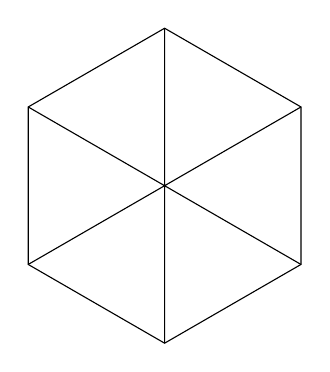
\begin{tikzpicture}[scale=2]
  % hexagon vertices
  \coordinate (A) at (0,1);
  \coordinate (B) at ({sqrt(3)/2},0.5);
  \coordinate (C) at ({sqrt(3)/2},-0.5);
  \coordinate (D) at (0,-1);
  \coordinate (E) at ({-sqrt(3)/2},-0.5);
  \coordinate (F) at ({-sqrt(3)/2},0.5);
  \coordinate (O) at (0,0);

  % outer hexagon
  \draw (A)--(B)--(C)--(D)--(E)--(F)--cycle;

  % subdivision into 6 triangles
  \draw (O)--(A) (O)--(B) (O)--(C)
        (O)--(D) (O)--(E) (O)--(F);
\end{tikzpicture}
		\end{center}
		Then $\chi(X) = 1$. Since we require that distinct regions of our hexagons have no more than one side in common, our hexagons must only be joined along their boundaries. An example of this would be:
		\begin{center}
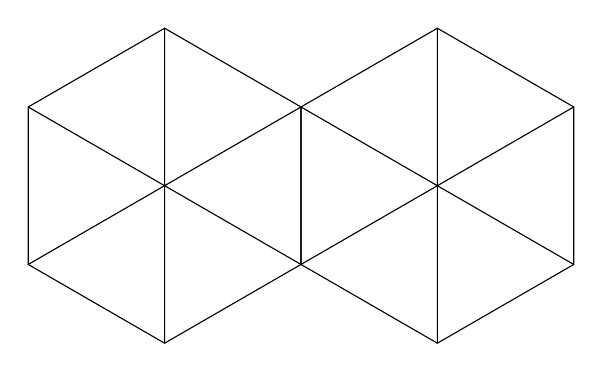
\begin{tikzpicture}[scale=2]
  % left hexagon
  \coordinate (O1) at (0,0);
  \coordinate (A1) at (0,1);
  \coordinate (B1) at ({sqrt(3)/2},0.5);
  \coordinate (C1) at ({sqrt(3)/2},-0.5);
  \coordinate (D1) at (0,-1);
  \coordinate (E1) at ({-sqrt(3)/2},-0.5);
  \coordinate (F1) at ({-sqrt(3)/2},0.5);

  % right hexagon, sharing edge B1--C1
  \coordinate (O2) at ({sqrt(3)},0);
  \coordinate (A2) at ({sqrt(3)},1);
  \coordinate (B2) at ({3*sqrt(3)/2},0.5);
  \coordinate (C2) at ({3*sqrt(3)/2},-0.5);
  \coordinate (D2) at ({sqrt(3)},-1);

  % outlines
  \draw (A1)--(B1)--(C1)--(D1)--(E1)--(F1)--cycle;
  \draw (A2)--(B2)--(C2)--(D2)--(C1)--(B1)--cycle;

  % subdivision into triangles
  \draw (O1)--(A1) (O1)--(B1) (O1)--(C1)
        (O1)--(D1) (O1)--(E1) (O1)--(F1);

  \draw (O2)--(A2) (O2)--(B1) (O2)--(B2)
        (O2)--(C2) (O2)--(C1) (O2)--(D2);
\end{tikzpicture}
		\end{center}
		The Euler characteristic of this triangulation can be computed as follows: we sum the Euler characteristics of each hexagon, and since we identify one edge together and two vertices together, the Euler characteristic of this triangulation is:
		\begin{align*}
			\chi(X) + \chi(X) - 2 - (-1)
			&= 1 \\
			&= 2 \cdot \chi(X) - 1 \\
		\end{align*}
		A simple induction argument will show that $n$ hexagons connected similarly as above has an Euler characteristic of $n \chi(X) - (n-1) = 1$. This is the largest possible Euler characteristic of a tiling of hexagons which do not overlap. If we were to tile hexagons which share more than one boundary in common, then we will always lose more vertices than edges. Hence any tiling of non-overlappping hexagons has an Euler characteristic of at most 1. But the Euler charactertic of a sphere is 2, hence it is not possible to subdivide the surface of a sphere with such a tiling.
	\end{proof}
%%%%%%%%%%%%%%%%%%%%%%%%%%%%%%%%%%%
%%%%%%%%%%%%%%%%%%%%%%%%%%%%%%%%%%%
%%%%%%%%%%%%%%%%%%%%%%%%%%%%%%%%%%%
\begin{exercise}[manual-num={3}]
	What surface is represented by a 10-gon with edges identified in pairs, as indicated by the symbol:
	\[
		abcdec^{-1}da^{-1}b^{-1}e^{-1}.
	\] 
\end{exercise}
	\begin{proof}
		Label each edge of the 10-gon by the ordering of the symbol. Label each vertex inbetween as $V_1,\ldots,V_{10}$. The Euler characteristic can be described as the number of even cells minus the number of odd cells. The 10-gon is itself a 2-cell, and after associating each edge we are left with five 1-cells. Note that our associations of vertices are:
		\begin{align*}
a &: \; V_1 \mapsto V_2,\quad V_9 \mapsto V_8 \\
b &: \; V_2 \mapsto V_3,\quad V_{10} \mapsto V_9 \\
c &: \; V_3 \mapsto V_4,\quad V_7 \mapsto V_6 \\
d &: \; V_4 \mapsto V_5,\quad V_7 \mapsto V_8 \\
e &: \; V_5 \mapsto V_6,\quad V_1 \mapsto V_{10}
\end{align*}
		Hence $V_1 \sim V_9$, $V_9 \sim V_3$, etc. Chasing the associations will show that each vertex is associated with each other, hence our 10-gon only has a single vertex. Thus the Euler characteristic of our 10-gon is $1 - 5 + 1 = -3$.
	\end{proof}

\end{document}
